\documentclass[man]{apa6}
\usepackage{lmodern}
\usepackage{amssymb,amsmath}
\usepackage{ifxetex,ifluatex}
\usepackage{fixltx2e} % provides \textsubscript
\ifnum 0\ifxetex 1\fi\ifluatex 1\fi=0 % if pdftex
  \usepackage[T1]{fontenc}
  \usepackage[utf8]{inputenc}
\else % if luatex or xelatex
  \ifxetex
    \usepackage{mathspec}
  \else
    \usepackage{fontspec}
  \fi
  \defaultfontfeatures{Ligatures=TeX,Scale=MatchLowercase}
\fi
% use upquote if available, for straight quotes in verbatim environments
\IfFileExists{upquote.sty}{\usepackage{upquote}}{}
% use microtype if available
\IfFileExists{microtype.sty}{%
\usepackage{microtype}
\UseMicrotypeSet[protrusion]{basicmath} % disable protrusion for tt fonts
}{}
\usepackage{hyperref}
\hypersetup{unicode=true,
            pdftitle={Final Project: Group 3},
            pdfauthor={Shaina Trevino, Maria Schweer-Collins, Alejandra Garcia Isaza, \& Ernst-August Doelle},
            pdfkeywords={keywords},
            pdfborder={0 0 0},
            breaklinks=true}
\urlstyle{same}  % don't use monospace font for urls
\usepackage{graphicx,grffile}
\makeatletter
\def\maxwidth{\ifdim\Gin@nat@width>\linewidth\linewidth\else\Gin@nat@width\fi}
\def\maxheight{\ifdim\Gin@nat@height>\textheight\textheight\else\Gin@nat@height\fi}
\makeatother
% Scale images if necessary, so that they will not overflow the page
% margins by default, and it is still possible to overwrite the defaults
% using explicit options in \includegraphics[width, height, ...]{}
\setkeys{Gin}{width=\maxwidth,height=\maxheight,keepaspectratio}
\IfFileExists{parskip.sty}{%
\usepackage{parskip}
}{% else
\setlength{\parindent}{0pt}
\setlength{\parskip}{6pt plus 2pt minus 1pt}
}
\setlength{\emergencystretch}{3em}  % prevent overfull lines
\providecommand{\tightlist}{%
  \setlength{\itemsep}{0pt}\setlength{\parskip}{0pt}}
\setcounter{secnumdepth}{0}
% Redefines (sub)paragraphs to behave more like sections
\ifx\paragraph\undefined\else
\let\oldparagraph\paragraph
\renewcommand{\paragraph}[1]{\oldparagraph{#1}\mbox{}}
\fi
\ifx\subparagraph\undefined\else
\let\oldsubparagraph\subparagraph
\renewcommand{\subparagraph}[1]{\oldsubparagraph{#1}\mbox{}}
\fi

%%% Use protect on footnotes to avoid problems with footnotes in titles
\let\rmarkdownfootnote\footnote%
\def\footnote{\protect\rmarkdownfootnote}


  \title{Final Project: Group 3}
    \author{Shaina Trevino\textsuperscript{1}, Maria
Schweer-Collins\textsuperscript{1}, Alejandra Garcia
Isaza\textsuperscript{1}, \& Ernst-August Doelle\textsuperscript{1}}
    \date{}
  
\shorttitle{Title}
\affiliation{
\vspace{0.5cm}
\textsuperscript{1} University of Oregon}
\keywords{keywords\newline\indent Word count: X}
\usepackage{csquotes}
\usepackage{upgreek}
\captionsetup{font=singlespacing,justification=justified}

\usepackage{longtable}
\usepackage{lscape}
\usepackage{multirow}
\usepackage{tabularx}
\usepackage[flushleft]{threeparttable}
\usepackage{threeparttablex}

\newenvironment{lltable}{\begin{landscape}\begin{center}\begin{ThreePartTable}}{\end{ThreePartTable}\end{center}\end{landscape}}

\makeatletter
\newcommand\LastLTentrywidth{1em}
\newlength\longtablewidth
\setlength{\longtablewidth}{1in}
\newcommand{\getlongtablewidth}{\begingroup \ifcsname LT@\roman{LT@tables}\endcsname \global\longtablewidth=0pt \renewcommand{\LT@entry}[2]{\global\advance\longtablewidth by ##2\relax\gdef\LastLTentrywidth{##2}}\@nameuse{LT@\roman{LT@tables}} \fi \endgroup}


\DeclareDelayedFloatFlavor{ThreePartTable}{table}
\DeclareDelayedFloatFlavor{lltable}{table}
\DeclareDelayedFloatFlavor*{longtable}{table}
\makeatletter
\renewcommand{\efloat@iwrite}[1]{\immediate\expandafter\protected@write\csname efloat@post#1\endcsname{}}
\makeatother
\usepackage{lineno}

\linenumbers

\authornote{Add complete departmental affiliations for each
author here. Each new line herein must be indented, like this line.

Enter author note here.

Correspondence concerning this article should be addressed to Shaina
Trevino, Postal address. E-mail:
\href{mailto:my@email.com}{\nolinkurl{my@email.com}}}

\abstract{
Sign Up: One or two sentences providing a \textbf{basic introduction} to
the field, comprehensible to a scientist in any discipline.

Two to three sentences of \textbf{more detailed background},
comprehensible to scientists in related disciplines.

One sentence clearly stating the \textbf{general problem} being
addressed by this particular study.

One sentence summarizing the main result (with the words ``\textbf{here
we show}'' or their equivalent).

Two or three sentences explaining what the \textbf{main result} reveals
in direct comparison to what was thought to be the case previously, or
how the main result adds to previous knowledge.

One or two sentences to put the results into a more \textbf{general
context}.

Two or three sentences to provide a \textbf{broader perspective},
readily comprehensible to a scientist in any discipline.


}

\begin{document}
\maketitle

\section{Introduction}\label{introduction}

Alejandra will do depression and health disparities (short 1 parapraph)
Maria will do drug use onset and health disparities (short 1 paragraph)

\section{Methods}\label{methods}

Sign up:

We report how we determined our sample size, all data exclusions (if
any), all manipulations, and all measures in the study.

\subsection{Participants}\label{participants}

Sign up:

\subsection{Measures}\label{measures}

sign up:

\subsection{Data analysis}\label{data-analysis}

We used R (Version 3.5.1; R Core Team, 2018) for all our analyses. sign
up:

\section{Results}\label{results}

We should use inline code here sign up: Alejandra will do the
description of her plot (depression, health insurance coverage, visit to
mental health, broken down by ethnicities). Shaina will describe her
plot of drug use by ethnicities
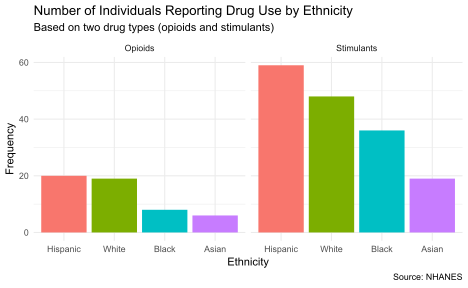
\includegraphics{Final_Paper_Group_3_files/figure-latex/ST_plot-1.svg}

\begin{figure}
\centering
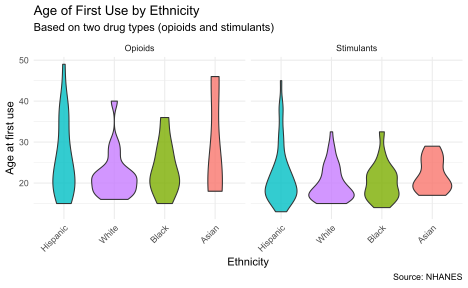
\includegraphics{Final_Paper_Group_3_files/figure-latex/ST_plot1-1.svg}
\caption{}
\end{figure}

\begin{verbatim}
## $title
## [1] "Association between Age at First Use and Depression"
## 
## $subtitle
## [1] "Colored to show differences among drug types"
## 
## $caption
## [1] "Source: NHANES"
## 
## $x
## [1] "Age at first use "
## 
## $y
## [1] "Total depression score"
## 
## attr(,"class")
## [1] "labels"
\end{verbatim}

\section{Discussion}\label{discussion}

sign up:

Insert one data visualization -- we are using two, I believe Alejandra's
viz. and one from Shaina Insert Table -- JP?

\newpage

\section{References}\label{references}

sign up: Alejandra will include the references used in the intro.

\begin{verbatim}
## Warning in utils::citation(x[pkg], auto = if (no_citations[pkg]) TRUE else
## NULL): no date field in DESCRIPTION file of package 'kableExtra'
\end{verbatim}

\begingroup
\setlength{\parindent}{-0.5in} \setlength{\leftskip}{0.5in}

\hypertarget{refs}{}
\hypertarget{ref-R-base}{}
R Core Team. (2018). \emph{R: A language and environment for statistical
computing}. Vienna, Austria: R Foundation for Statistical Computing.
Retrieved from \url{https://www.R-project.org/}

\endgroup


\end{document}
